% 图 71.1 —— 由 `checks/emit_hand.py` 自动拼出（probe 精测 + prims2 图元分解）
%%
% ⚠ 这是**稿子不是成品**：跑 `checks/checkhand.py 71.1` 看指标 + 看叠合图。
%%
%% ⚠ 待核：
%   · 本图 probe 报出阴影族 1 个 —— **本脚本不生成阴影**（要照原书手写）；prims2 的 strokes 里可能含阴影线，核对时留意别画重
%   · 可疑字形 2 项（空心圈 ⊙ 常被认成字母 o）—— 见文件末
%%
\documentclass[12pt]{standalone}
\usepackage{fontspec}
\setsansfont{Arial}
\newfontfamily\mfallback{DejaVu Sans}
\usepackage{tikz}
\begin{document}
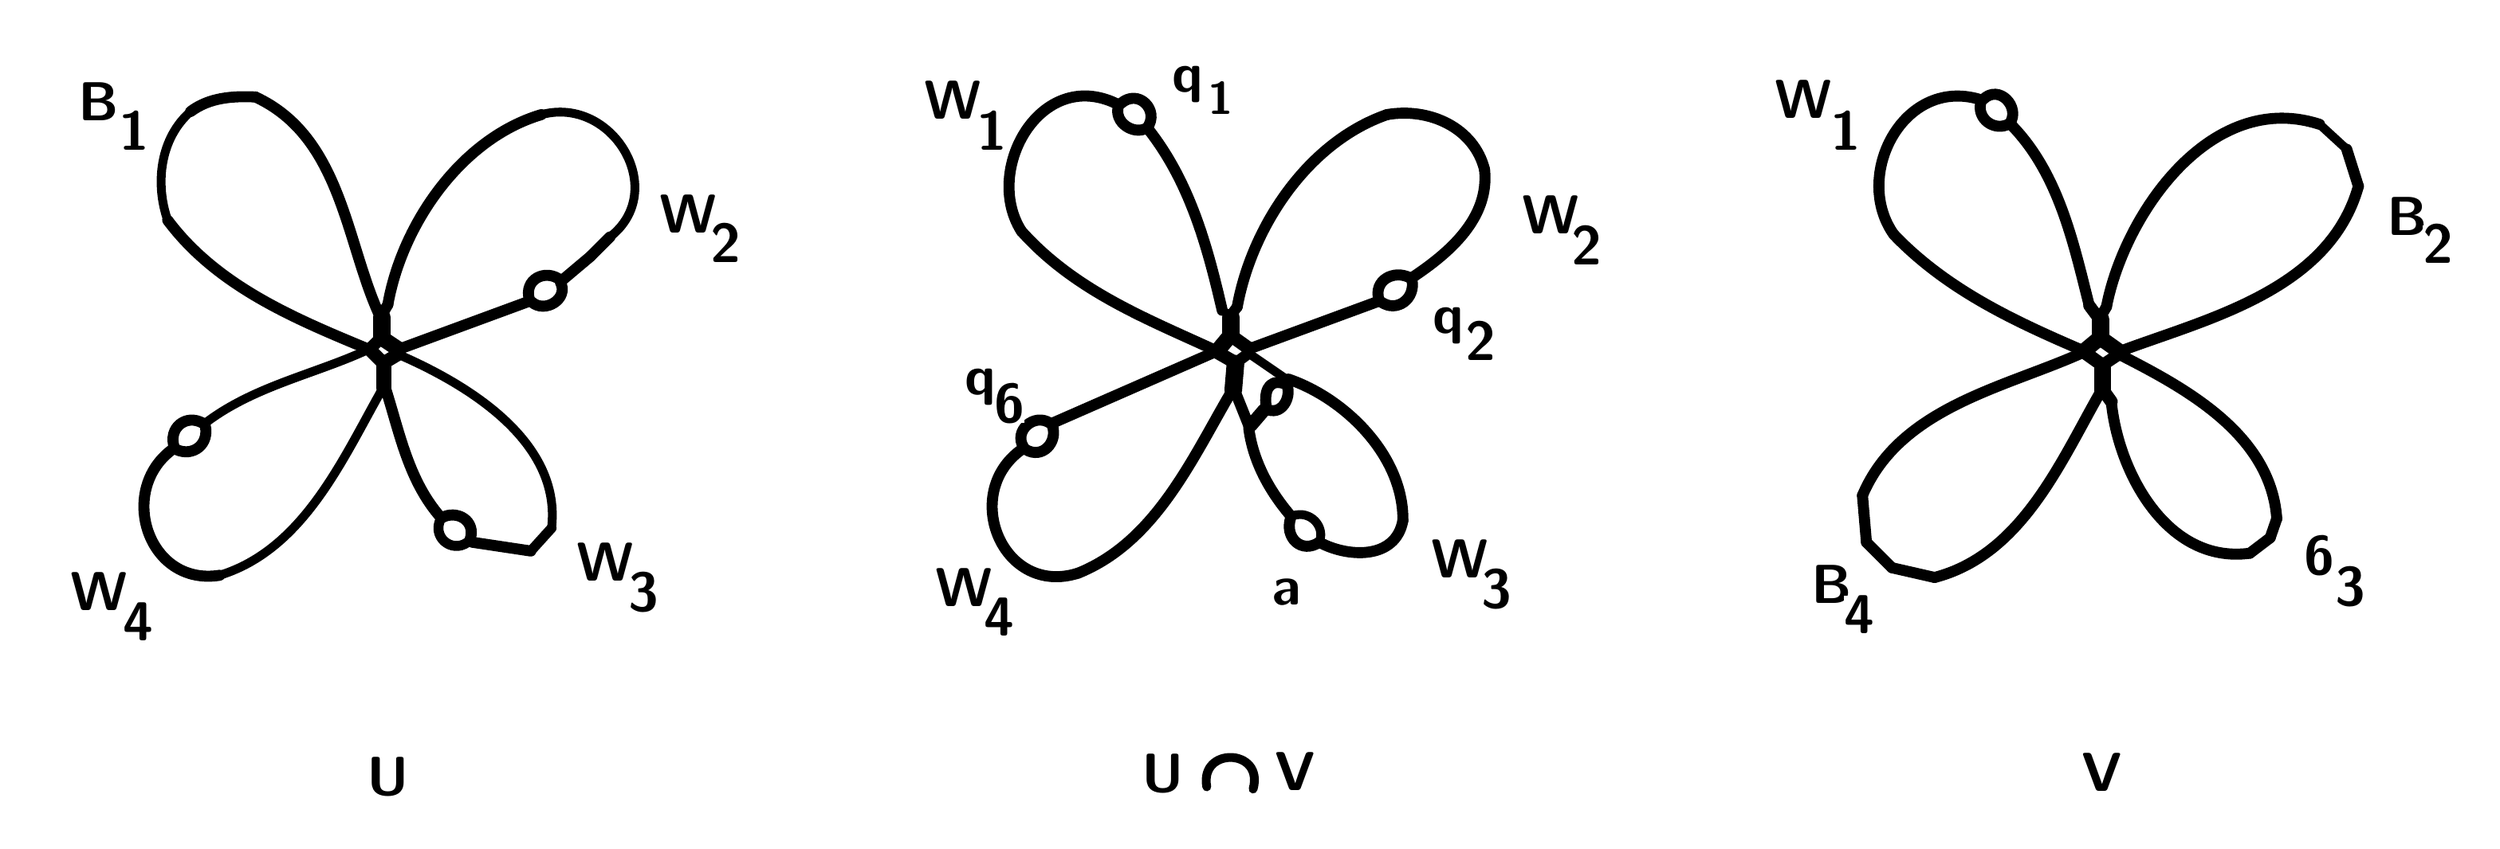
\begin{tikzpicture}[x=1pt, y=-1pt, line width=4.5pt, line cap=round, line join=round]

  %% ════ 直线段（prims2 的 strokes）════
  \draw[line width=4.5pt] (240.0,229.6) -- (230.6,240.0);
  \draw[line width=5.0pt] (230.6,240.0) -- (204.0,236.0);
  \draw[line width=5.1pt] (555.0,151.0) -- (551.0,154.0);
  \draw[line width=7.0pt] (943.0,144.0) -- (950.0,149.0);
  \draw[line width=5.0pt] (942.0,134.0) -- (944.8,129.2);
  \draw[line width=4.0pt] (1041.4,46.4) -- (1053.7,57.7);
  \draw[line width=5.0pt] (1053.7,57.7) -- (1059.0,74.5);
  \draw[line width=8.0pt] (163.0,143.0) -- (163.0,134.0);
  \draw[line width=5.0pt] (245.0,117.0) -- (257.7,106.3);
  \draw[line width=5.0pt] (257.7,106.3) -- (266.5,97.5);
  \draw[line width=5.0pt] (165.8,128.2) -- (163.0,133.0);
  \draw[line width=6.0pt] (158.0,149.0) -- (163.0,154.0);
  \draw[line width=5.0pt] (556.0,183.0) -- (550.0,168.0);
  \draw[line width=7.0pt] (542.0,149.0) -- (547.0,143.0);
  \draw[line width=5.0pt] (834.2,214.8) -- (836.0,236.0);
  \draw[line width=5.0pt] (836.0,236.0) -- (847.6,247.6);
  \draw[line width=5.0pt] (847.6,247.6) -- (866.9,252.0);
  \draw[line width=4.0pt] (557.0,151.0) -- (573.0,162.0);
  \draw[line width=6.0pt] (942.0,155.0) -- (935.0,150.0);
  \draw[line width=4.9pt] (550.8,129.2) -- (548.0,133.0);
  \draw[line width=7.0pt] (935.0,149.0) -- (941.0,144.0);
  \draw[line width=8.0pt] (548.0,142.0) -- (548.0,134.0);
  \draw[line width=5.5pt] (950.0,151.0) -- (944.0,155.0);
  \draw[line width=6.0pt] (549.0,143.0) -- (556.0,148.0);
  \draw[line width=7.5pt] (943.0,167.0) -- (943.0,156.0);
  \draw[line width=8.0pt] (942.0,143.0) -- (942.0,135.0);
  \draw[line width=5.0pt] (467.0,182.0) -- (540.0,150.0);
  \draw[line width=7.0pt] (164.0,155.0) -- (164.0,166.0);
  \draw[line width=7.0pt] (170.0,148.0) -- (164.0,144.0);
  \draw[line width=6.0pt] (165.0,154.0) -- (170.0,151.0);
  \draw[line width=6.0pt] (549.0,154.0) -- (542.0,150.0);
  \draw[line width=6.0pt] (557.0,183.0) -- (563.0,176.0);
  \draw[line width=5.0pt] (229.0,127.0) -- (172.0,148.0);
  \draw[line width=8.0pt] (550.0,155.0) -- (549.0,167.0);
  \draw[line width=3.8pt] (547.0,133.0) -- (544.0,130.8);
  \draw[line width=5.5pt] (941.0,134.0) -- (937.0,128.6);
  \draw[line width=5.5pt] (158.0,148.0) -- (162.0,144.0);
  \draw[line width=5.0pt] (1022.0,225.3) -- (1019.0,234.0);
  \draw[line width=5.0pt] (1019.0,234.0) -- (1009.8,241.0);
  \draw[line width=5.8pt] (947.0,172.2) -- (944.0,168.0);
  \draw[line width=5.0pt] (614.0,127.0) -- (557.0,148.0);

  %% ════ 曲线（prims2 的 curves —— 三段式，坐标同为 (y,x)）════
  \draw[line width=4.0pt] (171.0,151.0) .. controls (201.8,164.4) and (244.7,190.2) .. (240.0,229.6);
  \draw[line width=5.0pt] (453.0,194.0) .. controls (425.2,213.9) and (444.5,261.0) .. (478.8,250.0);
  \draw[line width=5.0pt] (478.8,250.0) .. controls (513.8,235.8) and (530.3,198.2) .. (548.0,168.0);
  \draw[line width=5.0pt] (944.8,129.2) .. controls (952.8,87.6) and (991.9,30.3) .. (1041.4,46.4);
  \draw[line width=5.0pt] (1059.0,74.5) .. controls (1045.9,121.5) and (990.9,134.5) .. (952.0,149.0);
  \draw[line width=4.0pt] (266.5,97.5) .. controls (293.4,76.5) and (267.8,33.3) .. (235.4,42.0);
  \draw[line width=5.0pt] (235.4,42.0) .. controls (199.0,52.8) and (172.2,91.8) .. (165.8,128.2);
  \draw[line width=5.0pt] (455.0,194.0) .. controls (462.4,198.4) and (469.6,190.8) .. (467.0,183.0);
  \draw[line width=5.0pt] (934.0,150.0) .. controls (899.1,165.8) and (851.2,174.6) .. (834.2,214.8);
  \draw[line width=5.0pt] (866.9,252.0) .. controls (906.4,241.7) and (923.9,199.7) .. (942.0,168.0);
  \draw[line width=5.0pt] (630.0,116.0) .. controls (646.7,104.9) and (665.3,89.1) .. (662.9,66.9);
  \draw[line width=5.0pt] (662.9,66.9) .. controls (658.1,47.8) and (637.8,38.7) .. (618.7,42.0);
  \draw[line width=5.0pt] (618.7,42.0) .. controls (582.5,54.6) and (557.3,93.3) .. (550.8,129.2);
  \draw[line width=5.0pt] (615.0,126.0) .. controls (612.5,117.0) and (621.9,112.3) .. (629.0,116.0);
  \draw[line width=4.0pt] (83.0,182.0) .. controls (104.8,165.3) and (132.2,159.9) .. (156.0,149.0);
  \draw[line width=5.0pt] (574.0,162.0) .. controls (599.8,170.8) and (626.2,196.9) .. (625.9,226.1);
  \draw[line width=5.0pt] (625.9,226.1) .. controls (622.6,244.3) and (600.6,242.9) .. (588.0,236.0);
  \draw[line width=5.0pt] (887.0,35.0) .. controls (852.5,25.0) and (829.5,70.0) .. (848.5,96.5);
  \draw[line width=5.0pt] (848.5,96.5) .. controls (872.8,121.8) and (903.8,136.0) .. (934.0,149.0);
  \draw[line width=5.0pt] (454.0,193.0) .. controls (449.2,185.4) and (458.9,177.2) .. (466.0,182.0);
  \draw[line width=5.0pt] (616.0,127.0) .. controls (623.2,132.0) and (631.7,125.5) .. (630.0,117.0);
  \draw[line width=4.0pt] (576.0,224.0) .. controls (584.0,221.3) and (590.9,229.0) .. (588.0,236.0);
  \draw[line width=5.0pt] (573.0,164.0) .. controls (575.7,168.9) and (571.9,178.2) .. (565.0,176.0);
  \draw[line width=4.0pt] (558.0,348.0) .. controls (563.1,329.4) and (533.6,328.7) .. (537.0,347.0);
  \draw[line width=5.0pt] (541.0,149.0) .. controls (510.0,134.7) and (477.4,122.1) .. (453.0,94.9);
  \draw[line width=5.0pt] (453.0,94.9) .. controls (435.4,67.4) and (461.5,20.4) .. (496.0,37.0);
  \draw[line width=5.0pt] (230.0,126.0) .. controls (227.2,116.8) and (237.1,111.8) .. (244.0,117.0);
  \draw[line width=5.0pt] (556.0,184.0) .. controls (557.8,198.8) and (565.1,212.4) .. (575.0,224.0);
  \draw[line width=5.0pt] (544.0,130.8) .. controls (537.3,101.8) and (529.3,72.2) .. (510.0,48.0);
  \draw[line width=5.0pt] (575.0,225.0) .. controls (572.1,234.1) and (580.1,241.4) .. (588.0,236.0);
  \draw[line width=5.0pt] (888.0,36.0) .. controls (885.5,43.9) and (894.3,50.1) .. (901.0,46.0);
  \draw[line width=5.0pt] (156.0,148.0) .. controls (123.8,134.6) and (88.4,119.9) .. (66.0,89.9);
  \draw[line width=4.0pt] (66.0,89.9) .. controls (60.2,73.4) and (62.5,52.7) .. (76.4,40.6);
  \draw[line width=5.0pt] (76.4,40.6) .. controls (84.8,34.3) and (95.2,33.5) .. (105.8,34.0);
  \draw[line width=5.0pt] (105.8,34.0) .. controls (144.8,52.1) and (146.7,99.7) .. (162.0,133.0);
  \draw[line width=5.0pt] (69.0,193.0) .. controls (66.1,184.2) and (74.2,177.6) .. (82.0,182.0);
  \draw[line width=5.0pt] (68.0,194.0) .. controls (43.0,212.6) and (57.1,256.2) .. (89.6,251.0);
  \draw[line width=4.0pt] (89.6,251.0) .. controls (127.5,239.3) and (145.2,198.5) .. (163.0,167.0);
  \draw[line width=5.0pt] (203.0,235.0) .. controls (206.1,226.3) and (197.1,221.0) .. (190.0,225.0);
  \draw[line width=4.5pt] (202.0,236.0) .. controls (194.6,241.3) and (185.3,233.4) .. (190.0,225.0);
  \draw[line width=5.0pt] (231.0,127.0) .. controls (237.0,132.4) and (248.0,125.5) .. (244.0,118.0);
  \draw[line width=5.0pt] (564.0,175.0) .. controls (563.0,169.0) and (564.1,161.6) .. (572.0,164.0);
  \draw[line width=5.0pt] (889.0,35.0) .. controls (896.2,28.1) and (905.9,38.6) .. (901.0,46.0);
  \draw[line width=5.0pt] (937.0,128.6) .. controls (929.7,99.7) and (923.0,68.0) .. (901.0,46.0);
  \draw[line width=5.0pt] (497.0,38.0) .. controls (494.6,45.5) and (503.9,51.6) .. (510.0,48.0);
  \draw[line width=5.0pt] (70.0,194.0) .. controls (77.6,197.4) and (85.0,191.5) .. (83.0,183.0);
  \draw[line width=5.0pt] (510.0,48.0) .. controls (515.8,40.1) and (506.0,29.9) .. (498.0,37.0);
  \draw[line width=5.0pt] (165.0,167.0) .. controls (171.3,187.0) and (175.3,208.4) .. (190.0,225.0);
  \draw[line width=5.0pt] (951.0,151.0) .. controls (980.8,166.2) and (1019.3,187.1) .. (1022.0,225.3);
  \draw[line width=5.0pt] (1009.8,241.0) .. controls (972.2,246.1) and (950.0,203.9) .. (947.0,172.2);

  %% ════ 标签（probe 直接给的 \node 行）════
  %% ⚠ 全部补了 fill=white：文字在最上层，否则与曲线交叉干扰
     \node[anchor=center,inner sep=0pt,fill=white,font=\fontsize{31.1}{38.9}\selectfont] at (528.5,28.3) {\textsf{\textbf{\textit{q}}}};   % box(519,15,17,23)
     \node[anchor=center,inner sep=0pt,fill=white,font=\fontsize{29.9}{37.4}\selectfont] at (422.2,35.5) {\textsf{\textbf{\textit{W}}}};   % box(409,23,26,23)
     \node[anchor=center,inner sep=0pt,fill=white,font=\fontsize{29.8}{37.2}\selectfont] at (807.7,35.0) {\textsf{\textbf{\textit{W}}}};   % box(794,23,27,22)
     \node[anchor=center,inner sep=0pt,fill=white,font=\fontsize{31.0}{38.8}\selectfont] at (34.8,36.0) {\textsf{\textbf{\textit{B}}}};   % box(23,24,20,23)
     \node[anchor=center,inner sep=0pt,fill=white,font=\fontsize{19.9}{24.9}\selectfont] at (543.3,34.8) {\textsf{\textbf{1}}};   % box(538,27,6,15)
     \node[anchor=center,inner sep=0pt,fill=white,font=\fontsize{23.7}{29.7}\selectfont] at (50.8,49.4) {\textsf{\textbf{1}}};   % box(44,41,8,16)
     \node[anchor=center,inner sep=0pt,fill=white,font=\fontsize{23.7}{29.7}\selectfont] at (439.8,49.4) {\textsf{\textbf{1}}};   % box(433,41,8,16)
     \node[anchor=center,inner sep=0pt,fill=white,font=\fontsize{23.7}{29.7}\selectfont] at (826.8,49.4) {\textsf{\textbf{1}}};   % box(820,41,8,16)
     \node[anchor=center,inner sep=0pt,fill=white,font=\fontsize{29.2}{36.6}\selectfont] at (302.2,87.0) {\textsf{\textbf{\textit{W}}}};   % box(289,75,26,22)
     \node[anchor=center,inner sep=0pt,fill=white,font=\fontsize{29.9}{37.4}\selectfont] at (693.2,87.5) {\textsf{\textbf{\textit{W}}}};   % box(680,75,26,23)
     \node[anchor=center,inner sep=0pt,fill=white,font=\fontsize{30.2}{37.8}\selectfont] at (1081.3,88.0) {\textsf{\textbf{\textit{B}}}};   % box(1070,76,19,23)
     \node[anchor=center,inner sep=0pt,fill=white,font=\fontsize{24.3}{30.4}\selectfont] at (319.1,100.4) {\textsf{\textbf{2}}};   % box(313,91,11,18)
     \node[anchor=center,inner sep=0pt,fill=white,font=\fontsize{24.3}{30.4}\selectfont] at (709.1,101.4) {\textsf{\textbf{2}}};   % box(703,92,11,18)
     \node[anchor=center,inner sep=0pt,fill=white,font=\fontsize{23.6}{29.6}\selectfont] at (1095.1,100.9) {\textsf{\textbf{2}}};   % box(1089,92,11,17)
     \node[anchor=center,inner sep=0pt,fill=white,font=\fontsize{30.5}{38.1}\selectfont] at (646.5,137.8) {\textsf{\textbf{\textit{q}}}};   % box(637,125,17,22)
     \node[anchor=center,inner sep=0pt,fill=white,font=\fontsize{23.6}{29.6}\selectfont] at (661.1,144.9) {\textsf{\textbf{2}}};   % box(655,136,11,17)
     \node[anchor=center,inner sep=0pt,fill=white,font=\fontsize{30.5}{38.1}\selectfont] at (434.5,165.8) {\textsf{\textbf{\textit{q}}}};   % box(425,153,17,22)
     \node[anchor=center,inner sep=0pt,fill=white,font=\fontsize{24.4}{30.5}\selectfont] at (447.6,173.1) {\textsf{\textbf{6}}};   % box(441,164,12,17)
     \node[anchor=center,inner sep=0pt,fill=white,font=\fontsize{36.5}{45.6}\selectfont] at (1041.4,241.9) {\textsf{\textbf{6}}};   % box(1031,229,19,24)
     \node[anchor=center,inner sep=0pt,fill=white,font=\fontsize{30.5}{38.1}\selectfont] at (651.8,243.5) {\textsf{\textbf{\textit{W}}}};   % box(638,231,27,23)
     \node[anchor=center,inner sep=0pt,fill=white,font=\fontsize{29.8}{37.2}\selectfont] at (264.7,245.0) {\textsf{\textbf{\textit{W}}}};   % box(251,233,27,22)
     \node[anchor=center,inner sep=0pt,fill=white,font=\fontsize{53.3}{66.7}\selectfont] at (573.3,258.7) {\textsf{\textbf{\textit{a}}}};   % box(558,242,27,28)
     \node[anchor=center,inner sep=0pt,fill=white,font=\fontsize{30.2}{37.8}\selectfont] at (820.3,255.0) {\textsf{\textbf{\textit{B}}}};   % box(809,243,19,23)
     \node[anchor=center,inner sep=0pt,fill=white,font=\fontsize{29.9}{37.4}\selectfont] at (427.2,256.5) {\textsf{\textbf{\textit{W}}}};   % box(414,244,26,23)
     \node[anchor=center,inner sep=0pt,fill=white,font=\fontsize{29.9}{37.4}\selectfont] at (35.2,258.5) {\textsf{\textbf{\textit{W}}}};   % box(22,246,26,23)
     \node[anchor=center,inner sep=0pt,fill=white,font=\fontsize{24.0}{30.0}\selectfont] at (1055.4,256.1) {\textsf{\textbf{3}}};   % box(1049,247,12,17)
     \node[anchor=center,inner sep=0pt,fill=white,font=\fontsize{24.0}{30.0}\selectfont] at (668.4,257.1) {\textsf{\textbf{3}}};   % box(662,248,12,17)
     \node[anchor=center,inner sep=0pt,fill=white,font=\fontsize{23.6}{29.5}\selectfont] at (281.9,258.6) {\textsf{\textbf{3}}};   % box(276,249,11,18)
     \node[anchor=center,inner sep=0pt,fill=white,font=\fontsize{23.5}{29.3}\selectfont] at (832.8,268.9) {\textsf{\textbf{4}}};   % box(826,260,12,17)
     \node[anchor=center,inner sep=0pt,fill=white,font=\fontsize{23.5}{29.3}\selectfont] at (442.8,269.9) {\textsf{\textbf{4}}};   % box(436,261,12,17)
     \node[anchor=center,inner sep=0pt,fill=white,font=\fontsize{23.5}{29.3}\selectfont] at (52.8,271.9) {\textsf{\textbf{4}}};   % box(46,263,12,17)
     \node[anchor=center,inner sep=0pt,fill=white,font=\fontsize{30.3}{37.9}\selectfont] at (517.0,340.8) {\textsf{\textbf{\textit{U}}}};   % box(507,328,20,23)
     \node[anchor=center,inner sep=0pt,fill=white,font=\fontsize{28.0}{35.0}\selectfont] at (577.3,339.9) {\textsf{\textbf{\textit{V}}}};   % box(569,328,17,22)
     \node[anchor=center,inner sep=0pt,fill=white,font=\fontsize{29.4}{36.8}\selectfont] at (942.8,340.5) {\textsf{\textbf{\textit{V}}}};   % box(934,328,18,23)
     \node[anchor=center,inner sep=0pt,fill=white,font=\fontsize{29.6}{37.0}\selectfont] at (166.0,342.2) {\textsf{\textbf{\textit{U}}}};   % box(156,330,20,22)

  % 钉死画布：否则超出的图元/控制点会把页面撑大，1:1 回比就失准
  \pgfresetboundingbox
  \path[use as bounding box] (0,0) rectangle (1113,365);
\end{tikzpicture}
\end{document}

% ⚠ 待核清单（probe 拿不准，人眼过一遍）：
%   · 未识别/跳过：⑤ 跳过/未识别的字形
%   · 未识别/跳过：box(536,332,25,18)
